% !TeX root = q1_v1.tex

\subsection{SURF}

Speeded-Up Robust Features (SURF) is another feature detection and description algorithm proposed by Herbert Bay, et al. in \cite{surf-original-bay}. This was also described in a more illustrated manner in \cite{surf-detailed-article-bay}. The primary contribution of the authors were exploiting the idea of integral image (which Voila and Jones originally proposed in \cite{voila-jones-cascade}), to speed up calculation of an approximated second order Gaussian (the Hessian matrix). The authors also proposed robust methods for descriptor extraction.

\paragraph*{Detector}

The keypoint detector has the following basic steps

\begin{enumerate}
    \item Estimate the integral image for the input image, using the equation below.

        \begin{equation*}
            I_{\sum}(\mathbf{x}) = \sum_{i=0}^{i \leq x} \sum_{j=0}^{j \leq y} I(i, j)
        \end{equation*}
    
    \item Approximate the terms in the hessian matrix: The determinant of hessian matrix is used as a proxy for feature points.
    Instead of using the Difference of Gaussian to estimate the terms in matrix, a second order approximation with simple terms is used.
    
        \begin{figure*}[h]
            \centering
            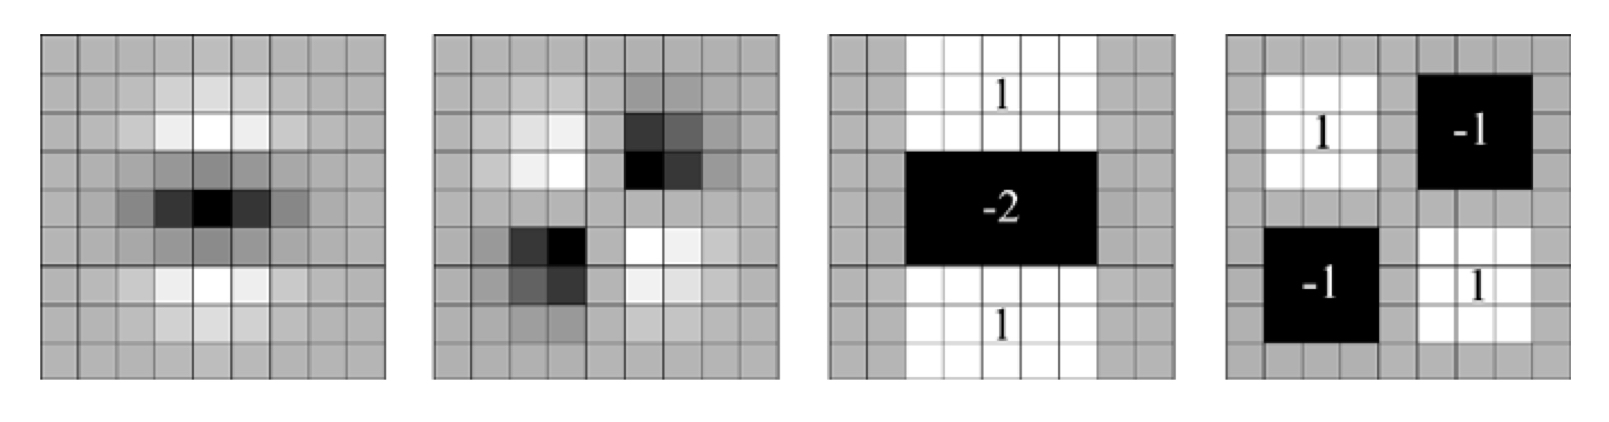
\includegraphics[width=0.5\textwidth]{surf_approx_dog.PNG}
            \caption{Approximation of second order derivatives}
            \small
                Left to right: Instead of $L_{yy}$ and $L_{xy}$ (first two), we use $D_{yy}$ and $D_{xy}$.
        \end{figure*}
    
    This approximation requires yields feature value as $\textup{det}(H_{approx}) = D_{xx} D_{yy} - (0.9 D_{xy})^2$. This is much faster to compute, but is still single scale

    \item Multiple scales: Instead of resizing the image, we can resize these kernels (as shown in the figure above). The standard sizes (to preserve center pixel) are $9\times 9$, $15\times 15$, $27\times 27$, \dots An octave consists of a series of filter response maps obtained using convolution with different filter sizes (set of four usually successive sizes).
    
    \item Non-Maximum Suppression: The maxima values in a $3\times 3\times 3$ neighborhood are retained and these are interpolated to their true scale and position on image.
\end{enumerate}

This yields the position of the keypoints; not just on the image, but also the particular scale of detection ($s$).

\paragraph*{Orientation alignment}

We need to obtain orientations before getting the descriptors. This is done in the following steps

\begin{enumerate}
    \item Calculate the \emph{Haar-wavelets} in the local region around the keypoint: We approximate the $dx$ and $dy$ filter (gradient in X and Y direction respectively) with a kernel containing $+1$ and $-1$ values. This is run on the $6s \times 6s$ neighborhood of the keypoint to get the gradients of neighboring points.

    \item Apply a gaussian weight with $\sigma=2s$
    
    \item Represent each point in the neighborhood as a point in a 2D scatter plot with X and Y values being the weighed $dx$ and $dy$ values.
    
    \item On this 2D scatter plot, run a window in polar form with the angle being $\sfrac{\pi}{3}$. Get the window with maximum sum (of weights of the points in the window).
    
    \item For this window, the orientation is calculated by summing the X and the Y values of the points (separately) and then getting the angle.
\end{enumerate}

We now have the orientation of each keypoint (thereby allowing us to get rotation robust descriptors). This orientation is also linked to the same scaling factor in which the keypoint was detected.

\paragraph*{Descriptor}

The descriptor is calculated in the following steps

\begin{enumerate}
    \item Get a $20s \times 20s$ oriented square patch around the keypoint (centered at the local feature). Calculate the integral image for this oriented patch, and estimate the Haar-wavelets (similar to the orientation alignment part) for $dx$ and $dy$ values for each pixel in this patch.

    \item Split this patch into $4\times 4$ sub-regions, with each sub-region having $5\times 5$ samples (actually, $5s\times 5s$ pixels).
    
    \item For each sub-region, calculate $\mathbf{v} = \left[\sum d_x, \sum \left | d_x \right |, \sum d_y, \sum \left | d_y \right | \right]$, a 4-dimensional descriptor of the particular sub-region.
    
    \item Stacking these 4-dimensional descriptors for every sub-region into a column vector gives the SURF descriptor. Invariance to contrast is achieved through normalizing them.
\end{enumerate}

The traditional SURF algorithm therefore gives a descriptor of length $4\times 4\times 4 = 64$. 

Despite being of smaller length, the descriptor (along with the matching method described in section 4.3 of \cite{surf-detailed-article-bay}) seems to give more robust correspondences than most other then-state-of-the-art methods. The authors demonstrate 3D reconstruction from un-calibrated cameras in section 5.2 of \cite{surf-detailed-article-bay}.
